\problemname{Upplega}

\begin{center}
\textit{''Ja, nu börjar det likna jul längs vägen\\ Överallt vi går''}
\end{center}

\noindent
Först när snön har lagt sig på alla grenar av de $N$ träden på gatan utanför ditt hus är det vinter på riktigt. 
Gatan med alla träd kan representeras i ett godtyckligt stort rutnät.
Längs med gatan står de $N$ träden på rad. Stammen av träd $i$ befinner sig på $pos_i$ och beskrivs av en
rektangel med bredd $1$ som tar upp hela kolumnen $pos_i$. Träd $i$ har dessutom $s_i$ grenar. Dessa grenar beskrivs vardera av en
rektangel som har höjd $1$ och sticker ut från stammen och är ett heltal längdenheter bred.
Det är garanterat att rutorna som varje gren befinner sig i inte överlappas av någon annan gren eller stam. 
Det är dessutom garanterat att ingen gren går förbi ett annat träd, ens ovanför det.

Efter en riktigt snöig afton har upplega lagt sig på alla träden. Upplega är benämningen på snö
som samlas på toppen av träds grenar. 
Ovanpå varje längdenhet av varje gren befinner det sig $1$ enhet snö. Snön är så tunn att den inte tar
upp en ruta. Detta innebär att snöns höjd är försumbar.

Du är en sann vinterentusiast som älskar jullåtar, det mysiga kalla vädret och framför allt all upplega. 
Enligt väderprognosen kommer det snart en stor storm, vilket kommer att skaka alla träd riktigt ordentligt. 
När ett träd blir skakat så kommer snön på dess grenar börja falla rakt ner till dess att snön antingen
landar säkert på en gren från ett träd som inte har blivit skakat eller att den hamnar på marken.
Trots att stormen snart ska börja hinner du skydda $K$ stycken träd från att skaka genom att rota träden.

Eftersom du gillar snö så mycket vill du beräkna största antalet enheter snö du kan förhindra från att
falla till marken genom att rota exakt $K$ stycken träd.

\begin{centering}
  \begin{figure}[h]
      \centering
      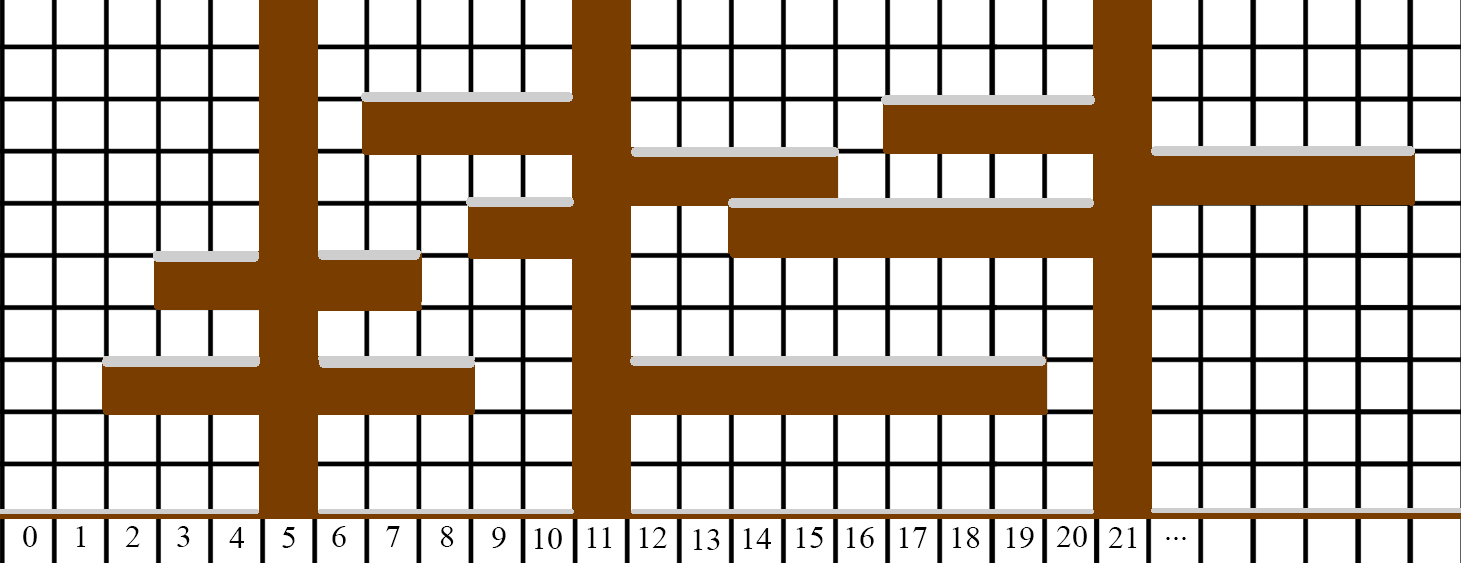
\includegraphics[width=0.8\textwidth]{sample1.png}
      \caption{Bilden visar exempelfall 1.}
  \end{figure}
\end{centering}

\section*{Indata}
Första raden innehåller två heltal $N$ och $K$ ($1 \leq K \leq N \leq 10^5$), antalet 
träd längs gatan och antalet träd som du hinner skydda från att skakas.

Andra raden innehåller $N$ heltal $pos_1, pos_2, \dots, pos_N$ ($0 \leq pos_i \leq 10^9$), där $pos_i$ är antalet längdenheter från början av gatan till träd $i$. 
Träden kommer att ges i sorterad ordning, och det är garanterat att inga två träd befinner sig på samma position. Formellt innebär det att om $i<j$ så gäller $pos_i < pos_j$.

Tredje raden innehåller $N$ heltal $s_1, s_2, \dots, s_N$ ($1 \leq s_i \leq 10$), där $s_i$ är antalet grenar som träd $i$ har. 

Till slut följer $2N$ rader, 2 rader per träd, som beskriver grenarna för trädet:
\begin{itemize}
  \item Första raden innehåller $s_i$ heltal $h_{i,1}, h_{i,2}, \dots, h_{i,s_i}$ ($1 \leq h_{i,j} \leq 10^9$) där $h_{i,j}$ är höjden på den $j$:te grenen som tillhör träd $i$. 
  \item Andra raden innehåller $s_i$ heltal $l_{i,1}, l_{i,2}, \dots, l_{i,s_i}$ ($-10^9 \leq l_{i,j} \leq 10^9$ , $l_{i,j} \neq 0$). 
  Varje $l_{i,j}$ beskriver längden och riktningen av gren $j$ som tillhör träd $i$. Om $l_{i,j}$ är positiv innebär det att gren $j$ riktas åt höger $l_{i,j}$ längdenheter. 
  Om $l_{i,j}$ är negativ riktas grenen $j$ åt vänster $|l_{i,j}|$ längdenheter.
\end{itemize}

Ingen gren kommer att befinna sig utanför gatans början som är vid $0$, eller befinna sig över $10^9$ längdenheter från början av gatan. 
%#2*N rows, 2 rows for each tree:
%h_1,h_2,...,h_{size_i}  %#given in a sorted ascending order, there can't be 2 branches on the exact same position, even from two different trees.
%l_1,l_2,...,l_{size_i} %#no branch will be so long that it will go outside [0,10^9]


\section*{Utdata}
Skriv ut det maximala antalet enheter snö som du kan från att att falla till marken genom att rota exakt $K$ stycken träd.

\section*{Poängsättning}
Din lösning kommer att testas på en mängd testfallsgrupper.
För att få poäng för en grupp så måste du klara alla testfall i gruppen.

\noindent
\begin{tabular}{| l | l | p{12cm} |}
  \hline
  \textbf{Grupp} & \textbf{Poäng} & \textbf{Gränser} \\ \hline
  $1$    & $5$        & Alla grenar pekar endast åt höger. Formellt gäller $l_{i,j} > 0$ för alla $i,j$.  \\ \hline
  $2$    & $5$        & $K = 1$ \\ \hline
  $3$    & $7$        & $N \leq 15$ \\ \hline
  $4$    & $11$       & $N \leq 2000, |l_{i,j}| \leq 2 \cdot 10^5, pos_i \leq 2 \cdot 10^5$ för alla $i,j$. \\ \hline %2000 or 1000 depending on how fast Python can solve it
  $5$    & $23$       & $N \leq 2000$  \\ \hline
  $6$    & $31$       & $ |l_{i,j}| \leq 2 \cdot 10^5, pos_i \leq 2 \cdot 10^5$ för alla $i,j$. \\ \hline
  $7$    & $18$       & Inga ytterligare begränsningar. \\ \hline
\end{tabular}

Grupp 4 och 6 garanterar också att alla träd och grenar befinner sig inom intervallet från $0$ till $4 \cdot 10^5$ längdenheter från början av gatan.

\section*{Explanation of sample 1:}
Genom att rota det första och andra trädet så förhindrar vi $10$ enheter snö från att falla från träd $1$, $18$ från träd $2$ och $9$ från träd $3$,
vilket sammanlagt blir $10+18+9=37$.
